\documentclass[a4paper,12pt]{article}
\usepackage{amsmath}
\usepackage[table,xcdraw]{xcolor}
\usepackage{graphicx}
\usepackage{amsmath}
\usepackage[bottom=2.0cm,top=3.0cm,left=3.0cm,right=2.0cm]{geometry}
\usepackage[brazilian]{babel}
\usepackage{indentfirst}
\usepackage{hyperref}  
\usepackage[nottoc]{tocbibind}
\usepackage{lipsum}
\usepackage{blindtext}
\usepackage{fontspec}
\usepackage[acronym, toc]{glossaries}
\usepackage{array}
\usepackage{multirow}
\usepackage{pdfpages}
\usepackage{tabularray}
\usepackage{siunitx}
\usepackage{float}
\usepackage{lscape}
\usepackage[table,xcdraw]{xcolor}
\usepackage{float}

\hypersetup{colorlinks,citecolor=black,filecolor=black,linkcolor=black,urlcolor=black}
\setmainfont{Arial}
\linespread{1.5}
\parindent=1cm
\makeglossaries

\newglossaryentry{tracker}{
    name=tracker,
    description={Um seguidor solar ou tracker é um dispositivo que altera várias vezes a posição dos painéis fotovoltaicos durante o dia, seguindo o caminho do sol para aumentar a produção de energia solar do sistema fotovoltaico}
}

\newglossaryentry{MVC}{
    name= MVC,
    description={MVC (Model-View-Controller) é um padrão de arquitetura de software que separa a aplicação em três componentes principais: o modelo (Model), a visualização (View) e o controlador (Controller). Esse padrão foi desenvolvido para melhorar a modularidade, a escalabilidade e a reutilização de código em aplicações web e desktop}
}
\newacronym{ncu}{NCU}{Network Control Unit}

\renewcommand{\labelenumii}{\theenumii}
\renewcommand{\theenumii}{\theenumi\arabic{enumii}.}

\begin{document}

\title{Requisitos para desenvolvimento}

\begin{titlepage}
	
    \begin{figure}[H]
        \begin{center}
            
\includegraphics[width=7cm]{logouf.png}
        \end{center}
    \end{figure}
	
	\begin{center}
        \vspace{-1cm}
        \large{\textbf{Universidade Federal da Paraíba - UFPB}}\\
        \large{Centro de Energias Alternativas e Renováveis - CEAR}\\
        \large{Departamento de Engenharia Elétrica - DEE}\\
        \large{Disciplina de Informática Industrial}\\
        
        \vspace*{\fill}
        \Large\textbf{Requisitos para desenvolvimento}
        \vspace*{\fill}
        
        \normalsize
        \hfill Grupo: \\
        \hfill Jaedson Barbosa Serafim \hspace{20pt} Mat: 20170024577\\\hspace{20pt} 
        \hfill Jose Helio Bento da Silva \hspace{20pt} Mat: 20180048133\\\hspace{20pt} 
        \hfill Fabiano de Souza Chaves Colaço \hspace{20pt} Mat: 20200093642  \newline
        
        \hfill Professor orientador:\\
        \hfill Ademar Virgolino da Silva Netto
        
        \vspace{\fill}
        João Pessoa - PB\\
        \today
          
	\end{center}
\end{titlepage}

\newpage

%\listoffigures
%\clearpage
\clearpage
\listoftables
\clearpage
\tableofcontents
\newpage
\pagenumbering{arabic}
\pagebreak

\section{Introdução}


A parceria da Huawei com a Universidade Federal Paraíba (UFPB) resultou na construção de uma usina fotovoltaica voltada para fins educacionais e econômicos no Centro de Informática, Campus I. A usina foi projetada tomando como modelo o parque solar de Coremas, possuindo 372 painéis conectados em doze strings, com capacidade máxima de 240kWp.

Com o intuito de maximizar a potência gerada, o projeto incluiu a capacidade das placas de ajustarem a sua inclinação para aumentar a incidência solar, a planta possui quatro \gls{tracker}s, cada um conectado à três strings.

São utilizados dois métodos para controlar a posição dos \gls{tracker}s, um comercial e outro desenvolvido por pesquisadores da UFPB. A solução comercial define a posição angular dos painéis a partir do horário, já a solução desenvolvida pelos pesquisadores utiliza uma inteligência artificial para ajustar a posição dos painéis para que maximize a potência gerada. Metade dos \gls{tracker}s utilizam a solução comercial e a outra a solução desenvolvida pelos pesquisadores.

Na planta são utilizados dois inversores SUN2000-100KTL-M1 de 100kW.  A ligação das strings nos inversores foi separada pela forma de controle da posição angular das strings, em um inversor são ligadas as strings controladas pelo método comercial e no outro inversor são conectadas as strings controladas pelo método desenvolvido pelos estudantes.
%colocar imagem
\begin{figure} [!h]
    \centering
    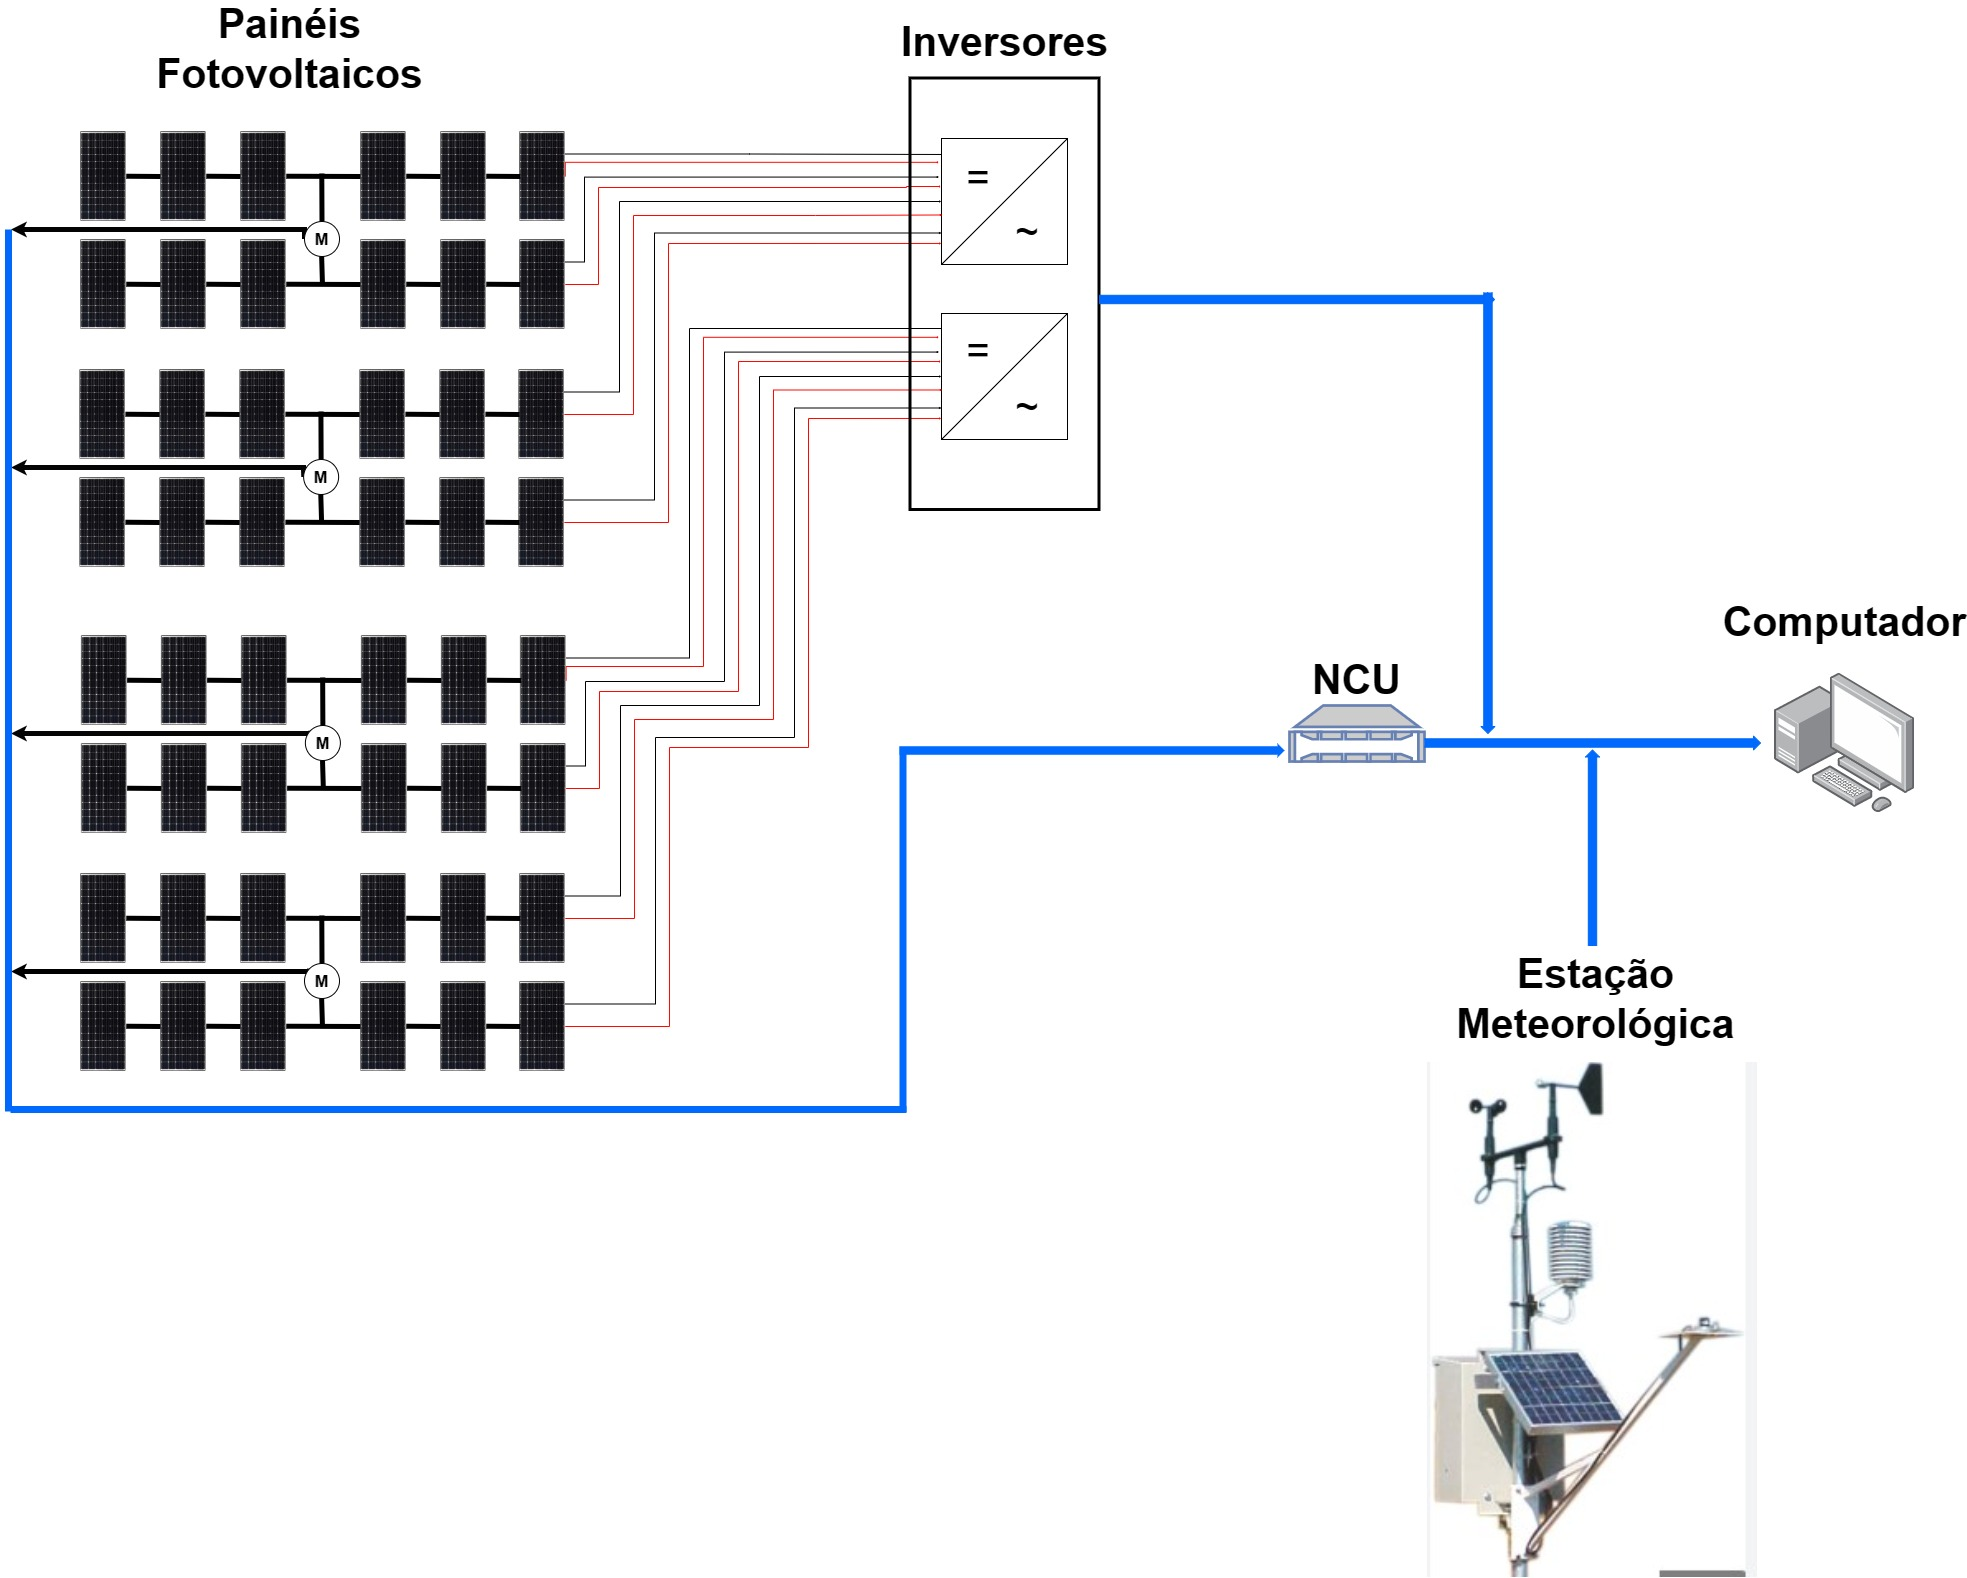
\includegraphics[width=15cm]{Imagem/Arquitetura_usina.jpg}
    \caption{Esquemático da usina fotovoltaica.}
    \label{fig: arquitetura_usina}
\end{figure}
% Continuar aqui


Além da parte relacionada com a geração da energia, existe uma estação meteorológica, entre os dados obtidos por ela temos: velocidade e direção do vento, temperatura, radiação total e difusa, umidade e precipitação da chuva. Esses dados são utilizados para o controle dos \gls{tracker}s, além disso, eles são armazenados em um banco de dados para futuras análises.

O controle da usina é feito através do \acrfull{ncu}, a comunicação entre ele e os demais componentes da usina (inversores, \gls{tracker}s e estação meteorológica) é feita através do protocolo de comunicação Modbus TCP IP como ilustrado na figura \ref{fig: arquitetura_usina}.

O sistema supervisório em funcionamento na usina, apesar de ser funcional, apresenta alguns problemas. Com o objetivo de resolver esses problemas e adicionar novas funcionalidades, será desenvolvido um novo um sistema supervisório para substituir o atual utilizado na planta. 

O novo sistema supervisório será implementado em um computador que se conectará com a usina através do protocolo de comunicação Modbus TCP IP, a partir dessa conexão ele será capaz de monitorar e obter dados da estação meteorológica, trackers e inversores. 

O acesso ao sistema será feito de forma exclusiva através de um sistema de login, onde apenas usuários registrados poderão acessar o sistema. Os usuários possuirão hierarquias diferentes, administrador, docente/operador, discente. O nível de hierarquia do usuário possibilitará, ou não, o acesso a funcionalidades específicas do sistema, como a alteração da posição dos trackers e o reconhecimento de alarmes.

O monitoramento da usina pelo operador será feito através de uma interface gráfica intuitiva composta por telas com funcionalidades específicas. A tela principal (sinótico) será responsável por exibir de forma resumida os dados importantes para o operador, como: alarmes, potência gerada por inversor, temperatura ambiente e posição dos trackers. As demais telas serão responsáveis por exibir de forma mais detalhada os dados contidos na tela principal.

Algumas telas serão personalizáveis, os dados exibidos nas telas poderão ser ajustados pelo operador de modo que seja possível comparar dados específicos em intervalos de tempos específicos, possibilitando a exibição de dados anteriores à data atual. 

A partir da análise dos dados, o sistema supervisório será capaz de quantificar o quanto foi gerado por string, por técnica de controle, total  e o ganho monetário. Ele também emitirá alertas caso a geração esteja abaixo do normal para condições climáticas semelhantes.

Além da visualização dos dados da usina, o operador também poderá tomar algumas ações, caso possua as permissões necessárias, como alterar a posição dos trackers, gerar relatórios personalizados e reconhecer alarmes.




\section{Requisitos}
\begin{enumerate}
    \item O sistema supervisório deve coletar dados dos inversores, trackers e estação meteorológica.
    \begin{enumerate}
        \item O sistema deverá se conectar via Modbus TCP IP com o NCU e com a estação meteorológica da usina.
        \item O sistema deve obter dos inversores a potência (kW), tensão (V) e corrente (A) por string e gerais. Esses dados devem ser identificados por inversor e por técnica de controle.
        \item O sistema deve obter da estação meteorológica os dados listados na tabela \ref{tab:dados-estacao}.
        \item O sistema deve obter dos trackers a tensão (V), corrente (A) e ângulo(°).
        \item Os dados deverão ser obtidos a cada dez segundos.
        \item A cada dez minutos deverá ser feita, para cada tipo de dado, uma média dos dados obtidos nesse intervalo, o valor será armazenado no banco de dados.
    \end{enumerate}
    
    \begin{table}[htbp]
\begin{center}
\begin{tabular}{|l|l|}
\hline
\textbf{Descrição} & \textbf{Unidade} \\
\hline
Radiação difusa & W/$m^2$ \\
Radiação total & W/$m^2$ \\
Direção do vento & graus \\
Velocidade do vento & m/s\\
Temperatura ambiente & °C\\
Precipitação da chuva & mm/$m^2$\\
Temperatura de uma placa & °C \\
\hline
\end{tabular}
\caption{Dados fornecidos pela estação meteorológica}
\label{tab:dados-estacao}
\end{center}
\end{table}


    \item Quantificar a energia gerada (kWh) e o rendimento (R\$) tanto por string quanto geral.
        \begin{enumerate}
            \item O sistema deve fornecer métricas, dos dados quantificados, de máxima, média e mínima nas escalas de tempo diária, mensal e anual.
            \item Essas métricas devem ser separadas por método de controle.
            \item Para cálculos das métricas nas escalas mensais e anuais, o sistema deve acessar os dados históricos.
        \end{enumerate}

    \item O sistema supervisório deve ter uma função de login/autenticação.
        \begin{enumerate}
            \item O sistema só poderá ser acessado por usuários registrados
            \item Os usuários possuirão nível de hierarquia diferentes, administrador, docente/operador e discente.
            \item O login será feito ao fornecer email/telefone e senha válidos
            \item O cadastro de novos usuários será feito pelo administrador
            \item Fornecer um sistema de autenticação com formulários de cadastro e de login via e-mail e/ou telefone; 
        \end{enumerate}

        \item Deve ter um função de Alarme cujas causas estão listadas na tabela \ref{tab:alarmes};
        \begin{enumerate}
            \item O sistema deve ser capaz de identificar as causas do alarme listadas na tabela \ref{tab:alarmes}.
            \item Deve emitir alertas visuais para chamar a atenção dos usuários;
            \item Deve conter um função que possibilite o usuário desativar o alarme quando a causa for resolvida.
            \item Deve enviar uma notificação por email para os usuários quando ocorrer um alarme.
        \end{enumerate}

        
\begin{table}[htbp]
\begin{center}
\begin{tabular}{|r|l|}
\hline
\textbf{Código} & \textbf{Descrição} \\
\hline
200 & Ângulo do tracker fora do limite de segurança\\
201 & Ângulo do tracker diferente do estabelecido\\
202 & Falha de comunicação com os inversores\\
203 & Falha de comunicação com os trackers\\
204 & Falha de comunicação com a estação meteorológica\\
202 & Falha interna nos inversores \\
203 & Velocidade do vento alta \\
204 & Subtensão no tracker X\\
205 & Sobrecorrente no tracker X\\
206 & Sobrecorrente no inversor X\\
\hline
\end{tabular}
\caption{Causas de alarmes}
\label{tab:alarmes}
\end{center}
\end{table}

    \item O sistema deve conter uma tela principal na qual será exibida os principais dados e gráficos de tendências
        \begin{enumerate}
            \item Deve mostrar se está sendo utilizada alguma técnica de backtracking.
            \item Deve ser mostrada a potência gerada por string, por inversor e total.
            \item Deve ter uma área para a exibição dos alarmes.
            \item Devem ser exibidos na tela a posição angular de cada tracker.
            \item Os dados que estão relacionados com o mesmo método de controle devem ser posicionados na tela de forma a deixar a visualização mais intuitiva.
             \item Devem ser exibidos na tela os seguintes dados meteorológicos: radiação difusa,direta, total, temperatura ambiente.
            \item A taxa de atualização da tela é de  10 segundos. Os dados mostrados serão a média dos dados obtidos nos últimos 10 minutos (precisa ser avaliado).
            \item Deve ser possível acessar as demais telas a partir da tela principal
            \item O acesso entre a tela principal e a demais telas deve ser projetada de maneira intuitiva. 
        \end{enumerate}
        
    \item O sistema deve ter uma tela para visualizar com mais detalhes os dados da tela principal. 
        \begin{enumerate}
            \item Nessa tela o usuário será capaz de escolher quais dados obtidos serão mostrados e o intervalo de tempo.
             \item O sistema deve conter recursos de visualização de dados que permitam o usuário analisar os padrões e tendências por meio de gráficos e tabelas.
            \item  O usuário deve ser capaz de personalizar os parâmetros exibidos na tela para atender às necessidades específicas do usuário.
            \item A taxa de atualização dessa tela deve ser o adequado para o usuário ter acesso às informações atualizadas.
             \item O sistema deve permitir que os usuários gerem relatórios no formato PDF baseado nos dados armazenados pelo supervisório.
             \item O sistema deve permitir que os usuários especifiquem os dados que desejam incluir no relatório e a ordem em que os dados devem ser apresentados.
            \item O sistema deve permitir exportar os dados em formato .xlsx e .csv para análises em outros softwares.
            \item O sistema deve gerar um pequeno relatório em um determinado intervalo de tempo para atualizar os usuários automaticamente.
        \end{enumerate}
        
    \item Deve conter uma tela para alarmes e dados históricos 
        \begin{enumerate}
            \item Deve ser possível reconhecer alarmes nessa tela.
            \item A tela deve incluir informações importantes como data e hora de um evento, como alarme ou alerta.
            \item O sistema deve permitir exportar os dados em formato .xlsx ou .csv para análises em outros softwares.
             \item O sistema deve conter um histórico de eventos  para armazenar ações ocorridas durante o processo e listadas na tabela \ref{tab:ocorrencias}
        \end{enumerate}

    \item O sistema deve analisar os dados de geração e avaliar a necessidade de manutenção
        \begin{enumerate}
            \item O sistema deve ser capaz de comparar os dados de geração com os dados previstos por meio dos dados meteorológicos e julgar a necessidade de manutenção.
            \item Deve emitir alertas para o usuário em caso da necessidade de manutenção.
        \end{enumerate}
    \item O sistema deve ser capaz de controlar o ângulo do tracker
        \begin{enumerate}
            \item O sistema deve permitir o usuário selecionar valores para o ângulo do tracker.
            \item Deve obter o ângulo atualizado do tracker para os usuários ajustar o ângulo de forma adequada.
            \item Deve ter um comando de controle para que o valor selecionado seja enviado para o tracker.
            \item A alteração do ângulo do tracker só poderá ser feita por usuários do tipo administrador/operador ou docente.
            \item  Deve visualizar o modo de operação do tracker.
            \item  Deve visualizar o ângulo setado e o medido.
        \end{enumerate}
    \item O sistema deve ter um banco de dados para armazenamento de dados pré-determinados de forma estruturada e clara.
\end{enumerate}


 \begin{table}[htbp]
\begin{center}
\begin{tabular}{|r|l|}
\hline
\textbf{Código} & \textbf{Descrição} \\
\hline
100 & Hora de ocorrência de um alarme \\
101 & Hora em que o alarme foi reconhecido \\
102 & Hora de impressão de relatório \\
103 & Hora de login e logout \\
104 & Hora de mudança \\
105 & Data da manutenção \\
\hline
\end{tabular}
\caption{Ocorrências a serem gravadas}
\label{tab:ocorrencias}
\end{center}
\end{table}   


\section {Modelos do sistema}
\subsection{Diagrama de caso de uso}

O modelo de caso de uso para o sistema supervisório é ilustrado na figura \ref{fig: caso de uso}. Ele ilustra que o usuário interage com o supervisório para acessar, visualizar e controlar ações no sistema "usina". Além disso, mostra que o sistema usina é uma generalização para os sistemas trackers, inversores e estação meteorológica.
%colocar imagem
\begin{figure} [htbp]
    \centering
    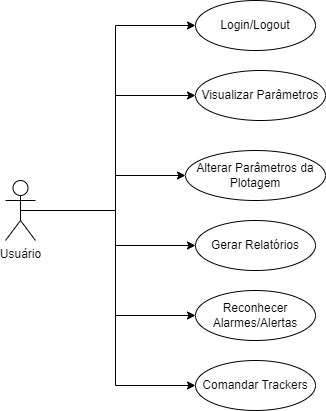
\includegraphics[width=15cm]{Imagem/Diagrama _caso_uso.png}
    \caption{Diagrama de caso de uso.}
    \label{fig: caso de uso}
\end{figure}
% Continuar aqui

Visando facilitar a compreensão quanto a funcionalidade, os detalhes como: atores,dados,estímulos e descrição são descritos nas tabelas a seguir para cada caso de uso.
\begin{table}[htbp]
\begin{center}
\begin{tabular}{|c|p{13cm}|}
\hline
\cellcolor{gray} \textbf{Caso de uso} &  Login/Logout\\
\hline
\cellcolor{gray} \textbf{Atores}  & Usuário \\
\hline
\cellcolor{gray} \textbf{Descrição} &   O usuário deve ser capaz de logar e sair do sistema.      \\
\hline
\cellcolor{gray} \textbf{Dados} &  email/telefone e senha \\ 
\hline
\cellcolor{gray} \textbf{Estímulos} & Comando do usuário \\
\hline
\cellcolor{gray} \textbf{Resposta} & Acesso ou não ao sistema. \\
\hline
\cellcolor{gray} \textbf{Comentários} & Sem comentários  \\
\hline
\end{tabular}
\caption{Descrição tabular para o caso de uso 'login/logout'}
\label{tab:login}
\end{center}
\end{table}


\begin{table}[htbp]
\begin{center}
\begin{tabular}{|c|p{13.2cm}|}
\hline
\cellcolor{gray} \textbf{Caso de uso} &   Visualizar Parâmetros\\
\hline
\cellcolor{gray} \textbf{Atores}  & Usuário \\
\hline
\cellcolor{gray} \textbf{Descrição} &   O usuário deve ser capaz visualizar os parâmetros essenciais de funcionamento da usina fotovoltaica, caso ele queira, ele poderá acessar os dados de forma mais detalhada em outra tela.     \\
\hline
\cellcolor{gray} \textbf{Dados} &  Dados dos trackers, inversores e estação meteorológica. \\ 
\hline
\cellcolor{gray} \textbf{Estímulos} & Comando do usuário \\
\hline
\cellcolor{gray} \textbf{Resposta} & Exibição dos dados essenciais sobre o funcionamento da usina.\\
\hline
\cellcolor{gray} \textbf{Comentários} &  O usuário deve ter as permissões adequadas para acessar o sistema.  \\
\hline
\end{tabular}
\caption{Descrição tabular para o caso de uso 'Visualizar parâmetros'}
\label{tab:visualizar_P}
\end{center}
\end{table}

\begin{table}[htbp]
\begin{center}
\begin{tabular}{|c|p{12cm}|}
\hline
\cellcolor{gray} \textbf{Caso de uso} &  Alterar Parâmetros da Visualização dos Dados\\
\hline
\cellcolor{gray} \textbf{Atores}  & Usuário \\
\hline
\cellcolor{gray} \textbf{Descrição} &   O usuário deve ser capaz de realizar as seguintes ações nas plotagens: Alterar a escala no eixo do tempo, adicionar/remover dados da plotagem, ampliar/reduzir determinada parte do gráfico.      \\
\hline
\cellcolor{gray} \textbf{Dados} &  Dados dos trackers, inversores e estação meteorológica. \\ 
\hline
\cellcolor{gray} \textbf{Estímulos} & Comando do usuário \\
\hline
\cellcolor{gray} \textbf{Resposta} & Uma mensagem de confirmação sutil deve aparecer na tela. \\
\hline
\cellcolor{gray} \textbf{Comentários} & O usuário deve ter as permissões adequadas para acessar o sistema.\\
\hline
\end{tabular}
\caption{Descrição tabular para o caso de uso 'Alterar parâmetros de plotagem'}
\label{tab:alterar_P}
\end{center}
\end{table}



\begin{table}[htbp]
\begin{center}
\begin{tabular}{|c|p{12cm}|}
\hline
\cellcolor{gray} \textbf{Caso de uso} &  Gerar relatórios\\
\hline
\cellcolor{gray} \textbf{Atores}  & Usuário \\
\hline
\cellcolor{gray} \textbf{Descrição} &   O usuário poderá gerar relatórios de potência, energia e rendimento e poderá definir a técnica de controle.      \\
\hline
\cellcolor{gray} \textbf{Dados} &  informações de geração e rendimento. \\ 
\hline
\cellcolor{gray} \textbf{Estímulos} & Comando do usuário \\
\hline
\cellcolor{gray} \textbf{Resposta} & relatório com os parâmetros potência, geração e rendimento. \\
\hline
\cellcolor{gray} \textbf{Comentários} & O usuário deve ter as permissões adequadas para acessar o sistema.\\
\hline
\end{tabular}
\caption{Descrição tabular para o caso de uso 'Gerar relatórios'}
\label{tab:gerar_R}
\end{center}
\end{table}



\begin{table}[htbp]
\begin{center}
\begin{tabular}{|c|p{12cm}|}
\hline
\cellcolor{gray} \textbf{Caso de uso} & Reconhecer alarmes e alertas\\
\hline
\cellcolor{gray} \textbf{Atores}  & Usuário \\
\hline
\cellcolor{gray} \textbf{Descrição} &  O usuário deverá receber sinais de alarmes e alertas caso haja alguma incompatibilidade no funcionamento da usina. Em caso de alarme, deverá agir e, quando solucionado, deverá parar o alarme.    \\
\hline
\cellcolor{gray} \textbf{Dados} &  strings \\ 
\hline
\cellcolor{gray} \textbf{Estímulos} & Identificação de  incompatibilidade no sistema \\
\hline
\cellcolor{gray} \textbf{Resposta} & Sinais de alarme e alerta em destaque na tela \\
\hline
\cellcolor{gray} \textbf{Comentários} & O usuário deve ter as permissões adequadas para acessar o sistema \\
\hline
\end{tabular}
\caption{Descrição tabular para o caso de uso 'Reconhecer alarmes e alertas}
\label{tab:reconhecer_a_a}
\end{center}
\end{table}



\begin{table}[htbp]
\begin{center}
\begin{tabular}{|c|p{12cm}|}
\hline
\cellcolor{gray} \textbf{Caso de uso} & Comandar Tracker\\
\hline
\cellcolor{gray} \textbf{Atores}  & Usuário \\
\hline
\cellcolor{gray} \textbf{Descrição} &  O usuário deve ser capaz de alterar o ângulo e o status do tracker (neve, vento forte, limpeza, descanso).   \\
\hline
\cellcolor{gray} \textbf{Dados} & posição, modo de operação e status do tracker  \\ 
\hline
\cellcolor{gray} \textbf{Estímulos} & Comando do usuário \\
\hline
\cellcolor{gray} \textbf{Resposta} & Confirmação de que o comando foi enviado para o tracker \\
\hline
\cellcolor{gray} \textbf{Comentários} & O usuário deve ter as permissões adequadas para acessar o sistema \\
\hline
\end{tabular}
\caption{Descrição tabular para o caso de uso 'comandar tracker'}
\label{tab:comandar_T}
\end{center}
\end{table}


\subsection{Diagramas de classe}

\begin{figure}
    \centering
    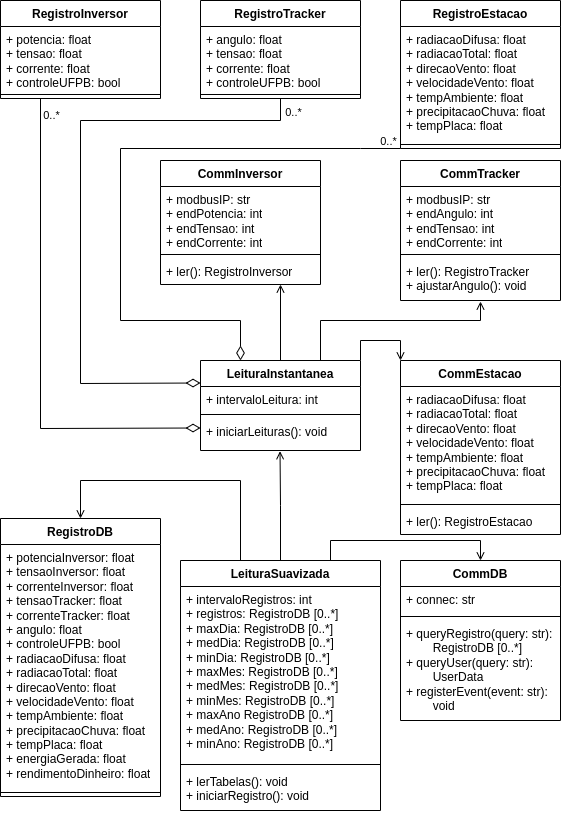
\includegraphics[width=\linewidth]{diagrama de classes.drawio.png}
    \caption{Diagrama de classes da camada \textit{Model}.}
    \label{fig:diagrama-classes-model}
\end{figure}

\begin{figure}
    \centering
    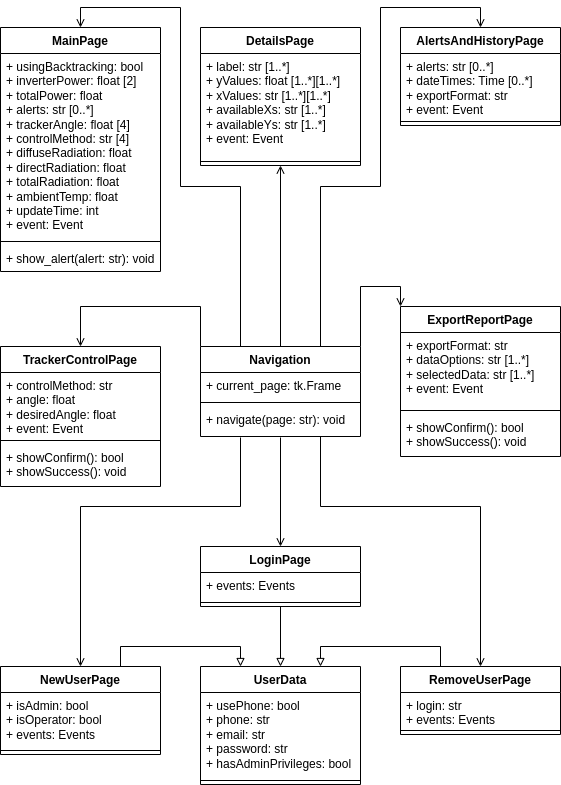
\includegraphics[width=\linewidth]{diagrama de classes - view.drawio.png}
    \caption{Diagrama de classes da camada \textit{View}.}
    \label{fig:diagrama-classes-view}
\end{figure}

\subsection{Diagrama de Sequências}

\section{Arquitetura do Sistema}
A arquitetura de alto nível para o sistema é ilustrada na figura \ref{fig: arquitetura_sistema}. O padrão de arquitetura escolhido para desenvolvimento do software é conhecido MVC por permitir a separação entre as alterações dos dados independente de sua representação. Neste modelo, o usuário irá interagir com o sistema por meio do "Controller" que enviará a interação do usuário para o View e Model, o View gerencia a forma como os dados são apresentados ao usuário, ou seja, a tela, já o Model é responsável pelo processamento dos dados.

O sistema supervisório irá se comunicar via TCP IP com a usina, cuja arquitetura é ilustrada na figura \ref{fig: arquitetura_usina}, para fazer requisições ou enviar dados ao computador. Já o computador faz requisições ao NCU e, no caso de controle do ângulo pelo usuário, enviará dados para o NCU.
%colocar imagem
\begin{figure} [htbp]
    \begin{center}
            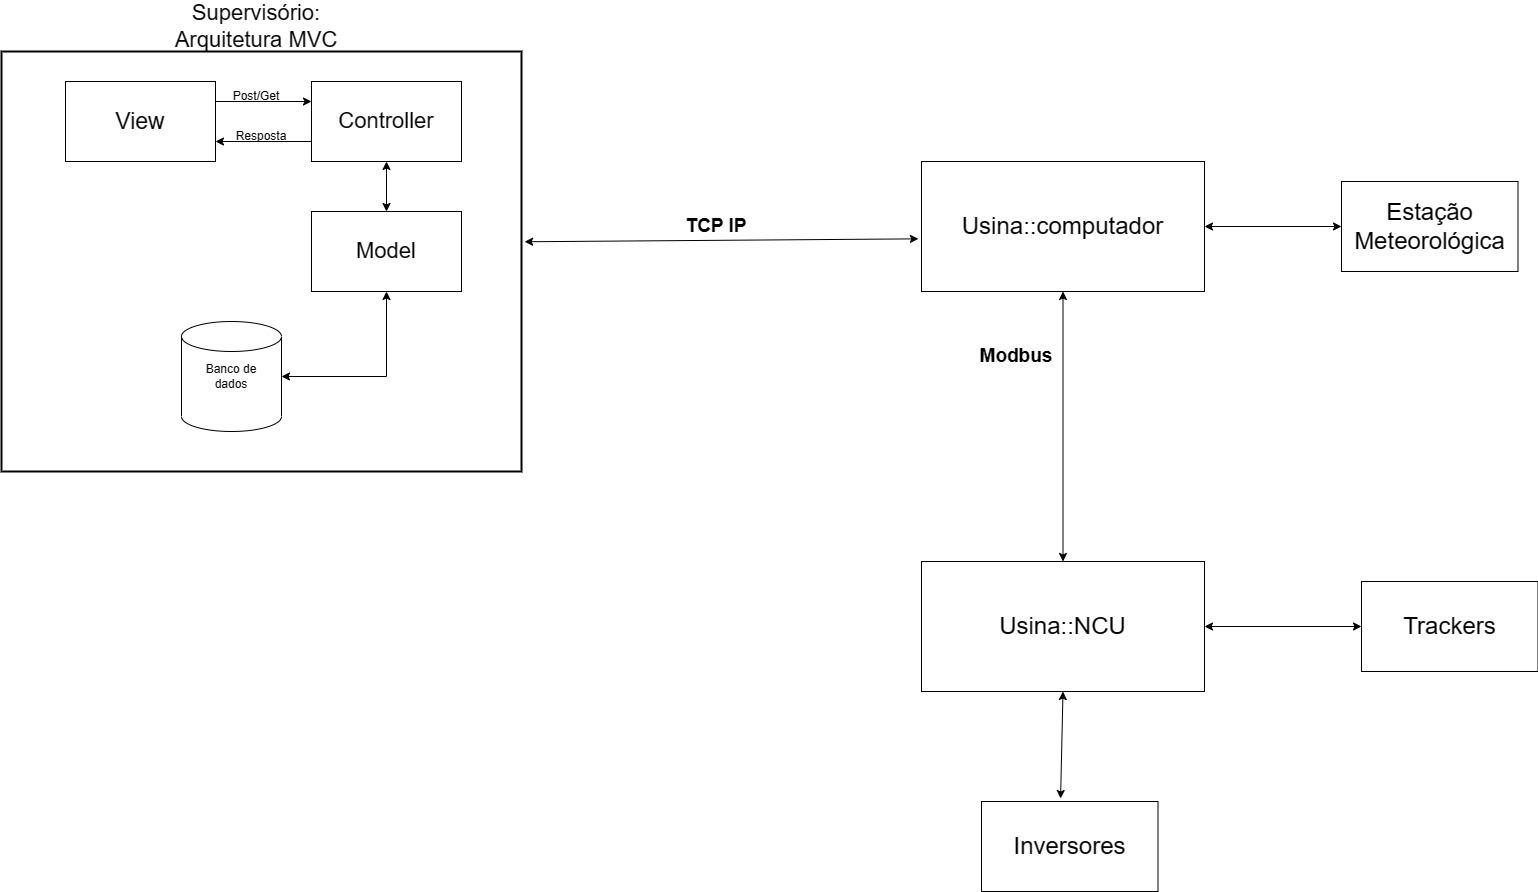
\includegraphics[width=15.5cm]{Imagem/arquitetura_sistema.jpg}
    \caption{arquitetura do sistema.}
    \label{fig: arquitetura_sistema}

    \end{center}
\end{figure}
% Continuar aqui

\clearpage
\printglossary[type=\acronymtype]
\printglossary

\end{document}

% olhar se é 240KWp
% são considerados 1 string por fileira pra questão de organização, mas são projetados 1,5 strings.
% tentar colocar a opção de mudar o algoritmo de controle
% adiconar: rodar em windows, uso do elipse nos requisitos.
% atualizar o diagrama de caso de uso
% diagrama de sequencia, componente e tempo, caso de uso e classe
